\documentclass[a4paper,10pt]{article}
\usepackage[utf8]{inputenc}
\usepackage{tikz}
\usepackage{amsmath}
\usepackage{fullpage}

%opening
\title{Attaque du protocole de la Team Tom}
\author{par l'Equipe Stone Jaws}

\begin{document}

\maketitle

\section{Le protocole}

Considérons 3 rôles $i$, $r$, et $m$ (que l'on appellera respectivement initiateur, récepteur, et serveur). La sémantique (en utilisant les notations de \cite{cas}) de ce protocole est alors donnée par :
\begin{eqnarray*}
	TeamTom(i) & = & \{ (i,r,m, K, K_{mi}), \\
		& & \texttt{send}_1(i,m, \textrm{senc}(\langle K,r \rangle, K_{mi}) ), \\
		& & \texttt{recv}_3(r,i,  h(K) ) \}\\
\end{eqnarray*}
\begin{eqnarray*}
	TeamTom(r) & = & \{ (i,r,m, K_{mr}), \\
		& & \texttt{recv}_2(m,r, \textrm{senc}(\langle i,V \rangle, K_{mr}) ), \\
		& & \texttt{send}_3(r,i,  h(V ) )  \} \\
\end{eqnarray*}
\begin{eqnarray*}
	TeamTom(m) & = & \{ (i,r,m, K_{mr}, K_{mi}), \\
		& & \texttt{recv}_1(i,m, \textrm{senc}(\langle W,r \rangle, K_{mi}) ), \\
		& & \texttt{send}_2(m,r, \textrm{senc}(\langle i,W \rangle, K_{mr}) )  \} \\
\end{eqnarray*}




\begin{figure}
\begin{center}
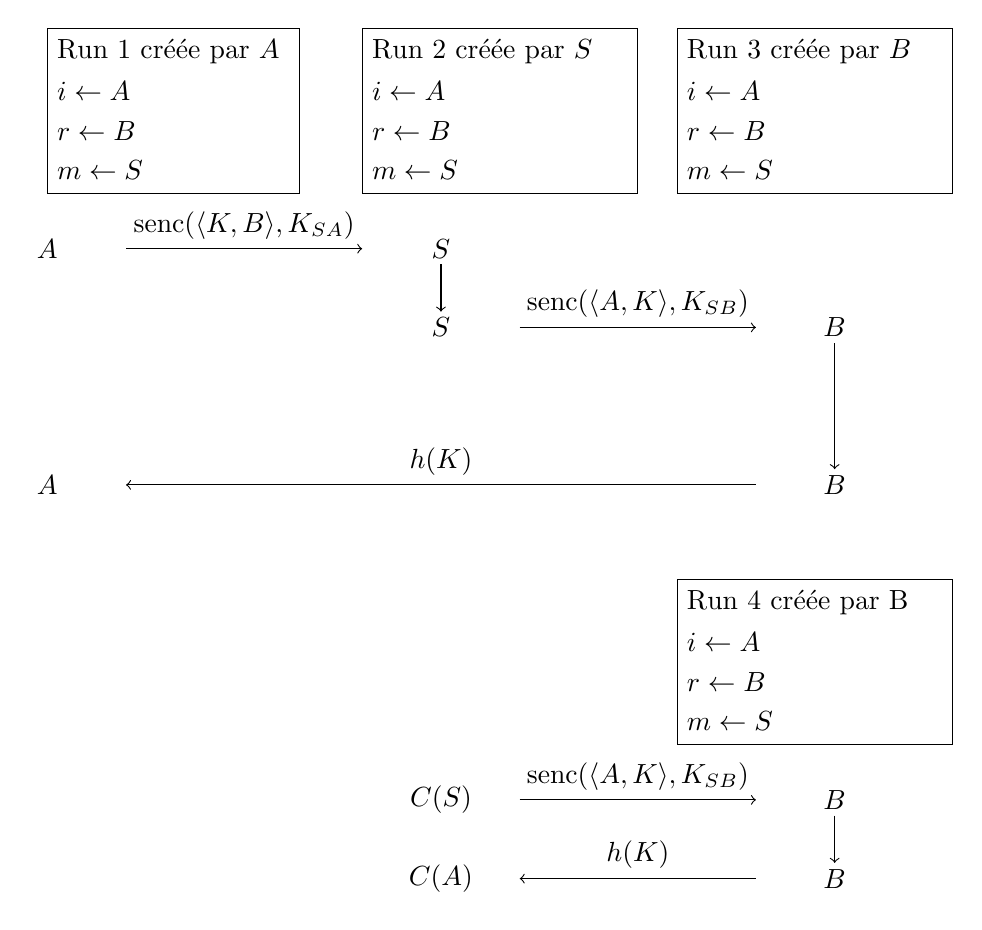
\begin{tikzpicture}
        \draw(-5,8.8) rectangle (-1.8,6.7);
	\draw (-5,8.5) node[right]{Run 1 créée par $A$};
	\draw (-5,8) node[right]{$i \leftarrow A$};
	\draw (-5,7.5) node[right]{$r \leftarrow B$};
	\draw (-5,7) node[right]{$m \leftarrow S$};
	\draw(3,8.8) rectangle (6.5,6.7);
	\draw (3,8.5) node[right]{Run 3 créée par $B$};
	\draw (3,8) node[right]{$i \leftarrow A$};
	\draw (3,7.5) node[right]{$r \leftarrow B$};
	\draw (3,7) node[right]{$m \leftarrow S$};
	\draw(-1,8.8) rectangle (2.5,6.7);
	\draw (-1,8.5) node[right]{Run 2 créée par $S$};
	\draw (-1,8) node[right]{$i \leftarrow A$};
	\draw (-1,7.5) node[right]{$r \leftarrow B$};
	\draw (-1,7) node[right]{$m \leftarrow S$};
	\draw (-5,6) node{$A$} ;
	\draw[->]  (-4,6) -- node[above]{$\textrm{senc}(\langle K,B \rangle, K_{SA})$} (-1,6);
	\draw (0,6) node{$S$} ;
	\draw[->]  (0,5.8) -- (0,5.2) ;
	\draw (0,5) node{$S$} ;
	\draw[->]  (1,5) -- node[above]{$\textrm{senc}(\langle A,K \rangle, K_{SB})$} (4,5) ;
	\draw (5,5) node{$B$} ;
	\draw[->]  (5,4.8) -- (5,3.2) ;
	\draw (5,3) node{$B$} ;
	\draw[->]  (4,3) -- node[above]{$h(K)$} (-4,3) ;
	\draw (-5,3) node{$A$} ;
	\draw (3,1.8) rectangle (6.5,-0.3);
	\draw (3,1.5) node[right]{Run 4 créée par B};
	\draw (3,1) node[right]{$i \leftarrow A$};
	\draw (3,0.5) node[right]{$ r \leftarrow B$};
	\draw (3,0) node[right]{$m \leftarrow S$};
	\draw (0,-1) node{$C(S)$};
	\draw[->] (1,-1) -- node[above]{$\textrm{senc}(\langle A,K \rangle, K_{SB})$} (4,-1);
	\draw (5,-1) node{$B$};
	\draw[->] (5,-1.2) -- (5,-1.8);
	\draw (5,-2) node{$B$} ;
	\draw[->] (4,-2) -- node[above]{$h(K)$} (1,-2);
	\draw (0,-2) node{$C(A)$};
\end{tikzpicture}
\end{center}
\caption{Attaque du protocole de la Team Tom}
\label{fig1}
\end{figure}




\section{Attaque sur le protocole}
L'attaque est représentée sur la Figure \ref{fig1} et fonctionne comme suit : 
\begin{enumerate}
	\item Le protocole est exécuté une première fois par les agents honnêtes $A$, $B$ et $S$ dans les rôles respectifs de $i$, $r$ et $m$. L'attaquant enregistre le deuxième message envoyé, $\textrm{senc}(\langle A,K \rangle, K_{SB})$. 
\item Plus tard, l'attaquant, représenté par un agent $C$, renvoie ce même message à $B$ en se faisant passer pour $S$. L'agent $B$ croît alors que $A$ désire lui communiquer le message $K$ par l'intermédiaire de $S$.
\item $B$ répond alors en envoyant $h(K)$, et l'attaquant intercepte ce message.
\end{enumerate}

On remarque alors que la synchronisation injective n'est pas vérifiée dans la trace correspondante, car dans la run $4$, l'agent $B$ croit recevoir un message $K$ de la part de l'agent $A$. Celui-ci lui a préalablement envoyé le message $K$, mais $B$ l'a déjà reçu dans une run différente (la run $3$, en l'occurrence), et $A$ ne lui a pas renvoyé ce message.

\bibliographystyle{plain}
\bibliography{ref.bib}


\end{document}
